\documentclass{ieeetj}
\usepackage{cite}
\usepackage{amsmath,amssymb,amsfonts,amsthm,mathtools}
\usepackage{graphicx,color,xcolor}
\usepackage{booktabs,multirow,url,bm,siunitx}
\usepackage{algorithm}
\usepackage{algpseudocode}
\usepackage{hyperref}
\hypersetup{hidelinks=true}
\AtBeginDocument{\definecolor{tmlcncolor}{cmyk}{0.93,0.59,0.15,0.02}\definecolor{NavyBlue}{RGB}{0,86,125}}
\makeatletter \let\@revised\@empty \makeatother
\def\OJlogo{}\def\seclogo{}
\def\authorrefmark#1{\ensuremath{^{\textbf{#1}}}}
\newtheorem{theorem}{Theorem}
\renewcommand{\thetheorem}{S\arabic{theorem}}
\renewcommand{\thesection}{S\arabic{section}}
\renewcommand{\thetable}{S\arabic{table}}
\renewcommand{\thefigure}{S\arabic{figure}}
\renewcommand{\theequation}{S\arabic{equation}}

\begin{document}
\markboth{}{Anonymous et al.}
\title{Supplementary Material for Backbone-Modular Neuro-Symbolic Post-Correction for OCT Denoising}
\author{Anonymous Author(s)\authorrefmark{1}}
\affil{\authorrefmark{1} Anonymous Affiliation}
\corresp{Correspondence withheld for double blind review.}
\maketitle

This document holds the material that does not fit inside the page limit of the main paper. It adds
nothing to the claims. It gives the closed form of every clinical property, the proof of the second
theorem, the training algorithm, the full list of constants, the visual comparison for all four
backbones, and a note on a defect found and repaired during revision.

% generated from diagnostics_nafnet.json over 173 images
\newcommand{\LipTheory}{0.5489}
\newcommand{\LipMeasured}{0.4679}
\newcommand{\AllocMean}{0.727}
\newcommand{\AllocStd}{0.050}
\newcommand{\NImages}{173}
\newcommand{\CondMargin}{141}
\newcommand{\CondSigma}{147}
\newcommand{\BoundOK}{99}
\newcommand{\CalibRho}{-0.258}
\newcommand{\CalibAuse}{0.775}
\newcommand{\EdgeInvBack}{0.45}
\newcommand{\EdgeInvCorr}{0.49}
\newcommand{\WeakRetBack}{40.5}
\newcommand{\WeakRetCorr}{44.5}
\newcommand{\DarkFrac}{1.6}
\newcommand{\DarkChange}{0.0072}
\newcommand{\IlmShiftBack}{4.73}
\newcommand{\IlmShiftCorr}{4.28}
\newcommand{\RpeShiftBack}{9.93}
\newcommand{\RpeShiftCorr}{10.24}
\newcommand{\GlobalChange}{0.0107}
\newcommand{\AllocMin}{0.556}
\newcommand{\AllocMax}{0.794}
\newcommand{\AllocClamp}{0.00}
\newcommand{\SigmaRatio}{0.961}
\newcommand{\EtaT}{0.0010}
\newcommand{\EtaB}{-0.0003}


% generated from paper/main.aux, do not edit
\newcommand{\EqObjective}{1}
\newcommand{\EqConfidence}{2}
\newcommand{\EqFailure}{3}
\newcommand{\EqAllocation}{4}
\newcommand{\EqStability}{5}
\newcommand{\EqLipschitz}{6}
\newcommand{\EqAlpha}{7}
\newcommand{\EqGate}{8}
\newcommand{\EqApply}{9}
\newcommand{\EqCandidate}{10}
\newcommand{\EqEnergy}{11}
\newcommand{\EqBlend}{12}
\newcommand{\EqCnrBound}{13}
\newcommand{\EqLossFid}{14}
\newcommand{\EqLossClin}{15}
\newcommand{\EqLossPred}{16}
\newcommand{\EqLossCoop}{17}
\newcommand{\EqLossEdge}{18}
\newcommand{\EqLossReg}{19}

\section{Closed form of the six clinical properties}
\label{sec:supp_predicates}
Table~\ref{tab:predicates_full} gives the score and the failure map of every property, and the
expanded definitions of every subterm follow. All quantities are computed from the noisy input and
the backbone output alone. No clean reference is used at any point.

\begin{table*}[t]
\centering
\caption{Closed form of the six clinical properties. For each predicate, the table lists its clinical role, image-level score, and pixel-level failure map. larger $\mathbf{m}_i$ means stronger evidence that the corresponding property is locally unsatisfied. The expanded subterm definitions follow immediately below. Here $\bar e=\operatorname{mean}(e(x))$, $b_e=\mathbf{1}[e(x)>\bar e]$, $v(z)=\operatorname{mean}_w z$ is a depth profile, $\rho_h$ is 1-pixel horizontal autocorrelation, and $\operatorname{Var}_k$ is local variance over a $k\times k$ window.}
\label{tab:predicates_full}
\setlength{\tabcolsep}{3pt}
\footnotesize
\begin{tabular}{cp{0.18\textwidth}p{0.33\textwidth}p{0.28\textwidth}c}
\toprule
$P_i$ & Clinical role & Aggregate score $s_i$ & Failure map $\mathbf{m}_i$ & $\tau_i$ \\
\midrule
$P_1$ & Edge continuity &
$0.4\,c_{\text{cont}}+0.3\,c_{\text{efr}}+0.3\,c_{\text{ang}}$ &
$(1-\tilde e)(1-b_e)$, \ $\tilde e=e(x)/(e_{\max}+\varepsilon)$ &
0.6 \\
$P_2$ & Local contrast recovery &
$0.20\,s_{\text{range}}+0.35\,s_{\text{cnr}}+0.20\,s_{\text{var}}+0.25\,s_{\text{cov}}$ &
$[\operatorname{ReLU}(\bar\sigma-\sigma_9(x))/(\bar\sigma+\varepsilon)+0.3\,\mathbf{1}[\sigma_9(x)<0.01]]_{[0,1]}$ &
0.5 \\
$P_3$ & Flat-region smoothness &
$0.6\,q_{\text{var}}+0.4\,q_{\text{res}}$ &
$F \odot \sigma_5(x)/(\max \sigma_5(x)+\varepsilon)$ &
0.75 \\
$P_4$ & Structural coherence &
$0.4\,s_{\text{self}}+0.3\,s_{\text{reg}}+0.3\,s_{\text{vert}}$ &
$e(e(x))/(\max e(e(x))+\varepsilon)$ &
0.5 \\
$P_5$ & Speckle conformity &
$0.7\,\operatorname{mean}(\exp(-|cv-cv^\star|/0.15))+0.3\,\exp(-5|\rho_h(z)|)$ &
$1-\exp(-|cv-cv^\star|/0.15)$ &
0.3 \\
$P_6$ & Layer visibility &
$0.4\,s_{\text{clr}}+0.3\,s_{\text{dep}}+0.3\,s_{\text{smo}}$ &
$\operatorname{Var}_7(e(x))/(\max \operatorname{Var}_7(e(x))+\varepsilon)$ &
0.7 \\
\bottomrule
\end{tabular}
\end{table*}

{\footnotesize
\noindent\textbf{Expanded subterms in Table~\ref{tab:predicates}.}
\textbf{$P_1$.}
$c_{\text{cont}}=\langle\operatorname{erode}(\operatorname{dilate}(b_e)),b_e\rangle/(\|b_e\|_1+\varepsilon)$,
$c_{\text{efr}}=\exp(-5|r_e-0.2|)$ with
$r_e=\|\mathbf{1}[e(x)>1.5\bar e]\|_1/(\|\mathbf{1}[e(x)<0.5\bar e]\|_1+\varepsilon)$,
and $c_{\text{ang}}=\exp(-2\,\operatorname{mean}(\sigma_5(\theta(x))))$.
\textbf{$P_2$.}
$s_{\text{range}}=\operatorname{sigm}(10(\Delta_r-0.3))$, $\Delta_r=\max(x)-\min(x)$.
$s_{\text{cnr}}=\operatorname{sigm}(15(\bar\sigma-0.05))$, $\bar\sigma=\operatorname{mean}(\sigma_9(x))$.
$s_{\text{var}}=\max(0.2,\operatorname{sigm}(-20(v_\sigma-0.02)+2))$, $v_\sigma=\operatorname{Var}(\sigma_9(x))$.
$s_{\text{cov}}=\operatorname{sigm}(5(\gamma-0.4))$, $\gamma=\operatorname{mean}(\mathbf{1}[\sigma_9(x)>0.3\bar\sigma])$.
\textbf{$P_3$.}
$F=\mathbf{1}[e(x)<0.3\bar e]$,
$q_{\text{var}}=1-\langle F,\sigma_5(x)/(\sigma_5(y)+\varepsilon)\rangle/(\|F\|_1+\varepsilon)$,
and $q_{\text{res}}=\exp(-5\,\operatorname{mean}|y-x|)$.
\textbf{$P_4$.}
$s_{\text{self}}$ is the average Pearson correlation between $x$ and shifts $(0,2)$, $(2,0)$, and $(2,2)$.
$s_{\text{reg}}=\exp(-12\,\operatorname{mean}(e(e(x))))$.
$s_{\text{vert}}=\operatorname{clip}(\max |\nabla_z v(x)|/(8\,\operatorname{mean}|\nabla_z v(x)|),0,1)$.
\textbf{$P_5$.}
$z=\log(y+\varepsilon)-\log(x+\varepsilon)$,
$cv=\sigma_{15}(|z|)/(\mu_{15}(|z|)+\varepsilon)$,
and $cv^\star(d)$, where $d$ is the axial depth index, is the depth-wise Gamma-K target coefficient of variation used by the implementation.
\textbf{$P_6$.}
$s_{\text{clr}}=\operatorname{mean}(\operatorname{clip}(\max |\nabla_z v(x)|/(10\,\operatorname{mean}|\nabla_z v(x)|),0,1))$,
$s_{\text{dep}}=\operatorname{clip}(20\,\operatorname{Var}(v(x)),0,1)$,
and $s_{\text{smo}}=1-\operatorname{clip}(10\,\operatorname{mean}(\operatorname{Var}_z(\operatorname{mean}_w e(x))),0,1)$.

These are the implemented predicates. The maps $\mathbf{m}_i$ are the spatial quantities consumed by the negotiator and potential head, while the scores $s_i$ drive the rule activations.
}
\noindent The released code computes exactly these quantities. The relevant class is named
\texttt{EnhancedGTFreePredicates} and the speckle property is computed by
\texttt{PhysicsAccurateSpecklePredicate}.

\section{Proofs}
\label{sec:supp_proof}

\subsection{Proof of the allocation stability result}
\label{sec:supp_proof_stability}
This is the proof of Theorem~1 of the main paper (Allocation stability), repeated here in full.
Write $s_k = -1$ for $k \in \{1,5\}$ and $s_k = +1$ otherwise, so that the allocation equation of the
main paper reads $a(\mathbf{r}) = b + \sum_{k} s_k C_k w_k r_k$ with $b$ independent of $\mathbf{r}$,
where $\mathbf{r} = (r_1, \ldots, r_5) \in [0,1]^5$ is the vector of rule truth values at one pixel,
$C_k$ are the fixed budgets, and $w_k = \sigma(\theta_k)$ are the learned rule weights.

\begin{proof}
Subtracting two such expressions gives
\begin{equation*}
a(\mathbf{r}) - a(\mathbf{r}') = \sum_{k} s_k C_k w_k (r_k - r'_k).
\end{equation*}
Taking absolute values and applying the triangle inequality,
\begin{equation*}
\begin{split}
\big| a(\mathbf{r}) - a(\mathbf{r}') \big|
&\le \sum_{k} C_k w_k \, |r_k - r'_k| \\
&\le \Big( \sum_{k} C_k w_k \Big) \lVert \mathbf{r} - \mathbf{r}' \rVert_\infty ,
\end{split}
\end{equation*}
which is the stability bound of Definition~1 of the main paper with $L = \sum_k C_k w_k$ as claimed.
The bound is attained by taking $r_k - r'_k = s_k t$ for any $t$ small enough to keep both vectors in
the unit cube, since then every term of the sum has the same sign. Because each $C_k$ is positive and
each $w_k = \sigma(\theta_k)$ lies strictly in $(0,1)$, the sum is strictly less than
$\sum_k C_k = 0.75$.
\end{proof}

\subsection{Proof of the contrast margin result}
\label{sec:supp_proof_cnr}
This is the proof of Theorem~2 of the main paper, repeated here in full. Write
$\mu_\mathcal{T}$ and $\mu_\mathcal{B}$ for the mean over tissue and over background, and
$\sigma_\mathcal{B}$ for the standard deviation over background. Let $\mathbf{b}$ be the backbone
output, $\mathbf{q}$ the candidate, and $\hat{\mathbf{x}} = (1-w)\mathbf{b} + w\mathbf{q}$ the output
with $w \in (0,1]$.

\begin{theorem}[Contrast margin]
Let $\eta_\mathcal{T} = \mu_\mathcal{T}(\mathbf{q}) - \mu_\mathcal{T}(\mathbf{b}) \ge 0$ and let
$\eta_\mathcal{B} \ge \mu_\mathcal{B}(\mathbf{q}) - \mu_\mathcal{B}(\mathbf{b})$. If
$\sigma_\mathcal{B}(\mathbf{q}) \le \sigma_\mathcal{B}(\mathbf{b})$, that
$\sigma_\mathcal{B}(\mathbf{b}) > 0$, that the tissue and background sets are the same for all three
images, and that the bounded numerator is non negative, then
\begin{equation}
\mathrm{CNR}(\hat{\mathbf{x}}) \ge
\frac{\big(\mu_\mathcal{T}(\mathbf{b}) - \mu_\mathcal{B}(\mathbf{b})\big)
      + w\,(\eta_\mathcal{T} - \eta_\mathcal{B})}{\sigma_\mathcal{B}(\mathbf{b})} .
\end{equation}
\end{theorem}

\begin{proof}
The mean is linear, so over any fixed set of pixels the mean of a convex combination is the same
convex combination of the means. Applying this over the tissue set and over the background set,
\begin{align*}
\mu_\mathcal{T}(\hat{\mathbf{x}}) &= (1-w)\,\mu_\mathcal{T}(\mathbf{b}) + w\,\mu_\mathcal{T}(\mathbf{q})
 = \mu_\mathcal{T}(\mathbf{b}) + w\,\eta_\mathcal{T}, \\
\mu_\mathcal{B}(\hat{\mathbf{x}}) &= \mu_\mathcal{B}(\mathbf{b}) + w\,\eta_\mathcal{B}',
\end{align*}
where $\eta_\mathcal{B}' = \mu_\mathcal{B}(\mathbf{q}) - \mu_\mathcal{B}(\mathbf{b}) \le \eta_\mathcal{B}$
by hypothesis. Subtracting,
\begin{equation*}
\begin{split}
\mu_\mathcal{T}(\hat{\mathbf{x}}) - \mu_\mathcal{B}(\hat{\mathbf{x}})
&= \big(\mu_\mathcal{T}(\mathbf{b}) - \mu_\mathcal{B}(\mathbf{b})\big) + w\,(\eta_\mathcal{T} - \eta_\mathcal{B}') \\
&\ge \big(\mu_\mathcal{T}(\mathbf{b}) - \mu_\mathcal{B}(\mathbf{b})\big) + w\,(\eta_\mathcal{T} - \eta_\mathcal{B}),
\end{split}
\end{equation*}
which lower bounds the numerator.

For the denominator, every background pixel of $\hat{\mathbf{x}}$ is the same convex combination of
the corresponding pixels of $\mathbf{b}$ and $\mathbf{q}$. Treating the background pixel values as a
random variable and applying Minkowski's inequality to the centered variables,
\begin{equation*}
\begin{split}
\sigma_\mathcal{B}(\hat{\mathbf{x}}) &\le (1-w)\,\sigma_\mathcal{B}(\mathbf{b}) + w\,\sigma_\mathcal{B}(\mathbf{q}) \\
&\le (1-w)\,\sigma_\mathcal{B}(\mathbf{b}) + w\,\sigma_\mathcal{B}(\mathbf{b}) = \sigma_\mathcal{B}(\mathbf{b}),
\end{split}
\end{equation*}
using the hypothesis $\sigma_\mathcal{B}(\mathbf{q}) \le \sigma_\mathcal{B}(\mathbf{b})$ in the second
step. Dividing the lower bound on the numerator by the upper bound on the denominator gives the
claim. Since $w > 0$ in every branch of the blending rule, the bound is at least the baseline
contrast whenever $\eta_\mathcal{T} > \eta_\mathcal{B}$.
\end{proof}

\noindent The results section of the main paper reports how often each of the three hypotheses holds on the
test set, so the reader can see when the guarantee is active rather than assuming it always is.

\section{Training procedure and the full list of constants}
\label{sec:supp_training}

\subsection{Algorithm}
Algorithm~\ref{alg:supp_training} states the procedure. The backbone is frozen throughout and
receives no gradient. The first stage activates only the clinical terms, so the correctors learn a
useful direction. The second stage activates the fidelity term, so they learn how far to go.

\begin{algorithm}[t]
\caption{Training the wrapper.}
\label{alg:supp_training}
\begin{algorithmic}[1]
\Require frozen backbone $f_\theta$, paired training set, number of epochs $E$
\State initialise the wrapper parameters, set each property threshold to its literature value
\For{$e = 1$ to $E$}
  \For{each batch of crops}
    \State compute the backbone output, with no gradient to $\theta$
    \State compute the confidence map from the backbone features
    \State compute the six property scores and failure maps
    \State compute the gain, edge and strength proposals
    \State compute the five rule truth values
    \State compute the allocation
    \State compose the candidate, then evaluate the objective on it
    \State update the wrapper parameters with AdamW
  \EndFor
  \If{$e$ reaches the midpoint} activate the fidelity term \EndIf
\EndFor
\end{algorithmic}
\end{algorithm}

\subsection{Structural constants}
The main paper lists the constants that carry a design decision. Table~\ref{tab:supp_constants} lists
the remaining ones, which are structural and were not tuned.

\begin{table}[t]
\centering
\caption{Structural constants. None of these was tuned.}
\label{tab:supp_constants}
\footnotesize
\begin{tabular}{llp{0.42\columnwidth}}
\toprule
Constant & Value & Role \\
\midrule
gate steepness & 20 & sharpness of the background gate \\
failure sharpness & 10 & sharpness of the score to failure conversion \\
smoothing window & $3 \times 3$ & smoothing of the brightening term \\
erosion window & $5 \times 5$ & keeps background smoothing away from tissue \\
crop size & $96 \times 96$ & training crops \\
batch size & 4 & training batch \\
edge bound & $\pm 0.08$ & nominal bound of the additive branch \\
quarter resolution & $H/4 \times W/4$ & the gain network runs at this scale \\
\bottomrule
\end{tabular}
\end{table}

\subsection{What the paired data is used for}
Training uses paired data. The clean reference enters the fidelity term, the clinical term and the
supervision of the edge branch. Testing uses no clean image anywhere in the correction path. The six
properties are computed from the noisy input and the backbone output only, which is what allows them
to run on a scanner the method has never seen. The clean reference is used to score results, as in
any denoising study, and never to produce them.

\section{A defect found during revision, and its repair}
\label{sec:supp_defect}

We record this because the released code contains a switch that restores the earlier behavior, and a
reader who finds that switch deserves to know what it is for.

\subsection{What was wrong}
In the version of this work that was first submitted, the allocation was formed by adding the rule
contributions to a base level and then clipping the result to the unit interval. The positive
contributions could reach $0.884$ and $0.762$ on top of a base of $0.818$, so the value arriving at
the clip could be as large as $2.46$. The clip was therefore active at every pixel of every image and
the allocation was the constant one.

Two consequences follow. The rule layer had no influence on any output, since multiplying by one
changes nothing. And the derivative of a clip at its bound is zero, so no gradient reached the rule
parameters and they stayed at their initial values for the whole of training. We confirmed both
directly, by reading the allocation map out of the trained model and by comparing every rule
parameter in the saved weights against its initializer after 2082 optimizer steps.

\subsection{The repair}
The allocation is now a bounded weighted vote. Writing $r_k \in [0,1]$ for the truth value of rule
$k$ and $w_k \in (0,1)$ for its learned weight,
\begin{equation}
\begin{split}
a = {}& B_{\min} + (B_{\max}-B_{\min})\,\sigma(\beta) \\
     & - C_1 w_1 r_1 + C_2 w_2 r_2 + C_3 w_3 r_3 \\
     & + C_4 w_4 r_4 - C_5 w_5 r_5 ,
\end{split}
\end{equation}
with $B_{\min} = 0.25$, $B_{\max} = 0.50$ and budgets $C_1 = 0.15$, $C_2 = 0.25$, $C_3 = 0.15$,
$C_4 = 0.10$ and $C_5 = 0.10$. The budgets satisfy
\begin{equation}
B_{\max} + C_2 + C_3 + C_4 = 1, \qquad B_{\min} - C_1 - C_5 = 0 ,
\end{equation}
so the value lies in the unit interval before any clipping, for every input and every parameter
setting. Clipping is therefore never active, saturation is impossible rather than unlikely, and the
gradient reaches every rule parameter.

The repair also tightens the theory. Because the allocation is affine in the rule truth values with
signed coefficients and no clipping intervenes, the Lipschitz constant of Theorem~1 of the main paper
is attained rather than merely an upper bound.

This is also what the trained model shows and not only a property of the formula. Measured on the
released weights, the allocation now spans $\AllocMin$ to $\AllocMax$ with mean $\AllocMean$ and
standard deviation $\AllocStd$, and $\AllocClamp$ percent of pixels sit at either end of the clamp,
against the whole image before the repair, direct confirmation that no pixel saturates in practice.

\subsection{Reproducing the earlier behavior}
Setting the environment variable \texttt{LEGACY\_SATURATING\_ALLOCATION} to $1$ restores the original
computation exactly. We verified this against a copy of the pre revision source on twenty random
inputs, comparing the allocation maps for equality and the rule traces for agreement. Both matched.
The earlier numbers can therefore be recovered from the released code, which is why the switch exists.

\section{Leave one out procedure for the clinical properties}
\label{sec:supp_studies}

The results section of the main paper reports the contribution of each clinical property. The procedure is
a leave one out ablation. At test time, one property at a time is switched off by setting its score
to the satisfied value and its failure map to zero, and the whole test set is re evaluated with that
property held-out. This is the same kind of one at a time removal used for the rule constants and for
the components of the method, applied here to the six clinical properties instead.

\section{Full per cell spreads}
\label{sec:supp_full_spreads}

The results table of the main paper prints each clinical cell as a mean, with the robustness
test folded into the choice of bold, and drops the per seed spread to keep the table one page.
Table~\ref{tab:supp_full_spreads} here restores that spread for every cell, four backbones by three
blocks by six measures, each as mean plus or minus one standard deviation across three seeds,
generated directly from the same result files.

\begin{table*}[!tb]
\centering
\caption{Every clinical cell of Tables 4 and 5 of the main paper, with its full mean plus or minus one seed
standard deviation restored. Each cell here is the one those tables show as a mean alone, and bold marks a mean that exceeds
its spread.}
\label{tab:supp_full_spreads}
\setlength{\tabcolsep}{4pt}
\footnotesize
\begin{tabular}{lcccccc}
\toprule
Backbone & $\Delta$CNR & $\Delta$TCI & $\Delta$EPI & $\Delta$BS & $\Delta$ENL & $\Delta$SNR \\
\midrule
\multicolumn{7}{l}{\textit{PKU37 test set, 173 images}} \\
\midrule
NAFNet & +3.49 $\pm$ 0.19 & +1.91 $\pm$ 0.51 & +1.20 $\pm$ 0.02 & +3.89 $\pm$ 0.45 & +23.74 $\pm$ 0.38 & +11.10 $\pm$ 0.31 \\
DnCNN & +11.30 $\pm$ 0.52 & +0.99 $\pm$ 1.62 & +4.14 $\pm$ 0.16 & -1.44 $\pm$ 0.87 & +57.14 $\pm$ 7.63 & +22.95 $\pm$ 2.28 \\
SwinIR & +7.33 $\pm$ 0.81 & +11.45 $\pm$ 0.86 & +2.68 $\pm$ 0.16 & +1.82 $\pm$ 0.37 & +28.32 $\pm$ 1.30 & +11.54 $\pm$ 0.26 \\
KBNet & +6.93 $\pm$ 0.98 & +5.92 $\pm$ 1.81 & +0.00 $\pm$ 0.07 & +2.58 $\pm$ 1.35 & +25.30 $\pm$ 2.17 & +7.95 $\pm$ 0.36 \\
\midrule
\multicolumn{7}{l}{\textit{Duke17, no adaptation}} \\
\midrule
NAFNet & +7.51 $\pm$ 0.21 & +4.00 $\pm$ 1.08 & +1.37 $\pm$ 0.07 & +4.15 $\pm$ 0.16 & +21.35 $\pm$ 1.78 & +5.43 $\pm$ 0.80 \\
DnCNN & +12.19 $\pm$ 0.72 & -1.47 $\pm$ 3.15 & +3.49 $\pm$ 0.15 & -2.24 $\pm$ 1.55 & +39.42 $\pm$ 5.44 & +13.55 $\pm$ 1.35 \\
SwinIR & +8.68 $\pm$ 1.12 & +13.26 $\pm$ 0.91 & +2.69 $\pm$ 0.24 & +1.90 $\pm$ 1.00 & +29.46 $\pm$ 0.66 & +11.60 $\pm$ 0.29 \\
KBNet & +5.34 $\pm$ 0.87 & +7.19 $\pm$ 1.57 & -0.50 $\pm$ 0.19 & +1.61 $\pm$ 0.09 & +7.49 $\pm$ 3.76 & -1.81 $\pm$ 1.80 \\
\midrule
\multicolumn{7}{l}{\textit{Duke2013, no adaptation}} \\
\midrule
NAFNet & +7.37 $\pm$ 0.06 & +1.41 $\pm$ 0.87 & +0.85 $\pm$ 0.04 & +0.51 $\pm$ 0.16 & +28.80 $\pm$ 2.25 & +9.29 $\pm$ 1.25 \\
DnCNN & +12.73 $\pm$ 1.41 & -2.21 $\pm$ 2.71 & +2.99 $\pm$ 0.25 & -5.85 $\pm$ 0.87 & +49.91 $\pm$ 7.29 & +17.59 $\pm$ 2.04 \\
SwinIR & +9.26 $\pm$ 1.20 & +11.86 $\pm$ 1.10 & +2.55 $\pm$ 0.20 & +2.30 $\pm$ 1.69 & +30.90 $\pm$ 1.02 & +13.31 $\pm$ 0.20 \\
KBNet & +7.16 $\pm$ 0.94 & +4.83 $\pm$ 1.32 & -0.35 $\pm$ 0.09 & +3.06 $\pm$ 1.03 & +8.70 $\pm$ 4.55 & -0.90 $\pm$ 2.14 \\
\bottomrule
\end{tabular}

\end{table*}

\section{The cooperation map, in full}
\label{sec:supp_cooperation}

The main paper reports that the map produced by the head reading the backbone features does not
predict the error of that backbone. This section gives the rest of the analysis.

Two measures were computed over the \NImages{} test images. The quantity correlated with the
absolute error of the backbone output is the demand map $\mathbf{u} = \mathbf{1} - \mathbf{c}$, which
is high where the wrapper is told to act. A demand map that tracked backbone error would give a
positive correlation. The measured rank correlation is \CalibRho{}, so the ordering runs the other
way. The sparsification error, the area between the curve obtained by removing the pixels the map
calls least reliable and the curve obtained by removing the pixels that are actually worst, is
\CalibAuse{}. A perfect ordering scores zero on the second measure and one on the first.

The reason is structural rather than a matter of tuning. The head is trained only through the
cooperation term of the objective, which rewards agreement between the map and the estimated
correction potential. That potential is itself a learned quantity. A map supervised only against
another learned map has no path by which the error of the backbone could reach it, so there is no
reason for it to acquire the meaning the original name implied.

Repairing this would require a term that regresses the map on the measured backbone error. Such a
term would compete with the cooperation term rather than complement it, because one pulls the map
toward the error of the backbone and the other pulls it toward where the correctors want to act. The
relative weight of the two would have to be selected, and every result in this paper would have to be
recomputed. We therefore report the measurement and leave the repair as the clearest piece of future
work this revision has identified.

\begin{figure*}[!tb]
\centering
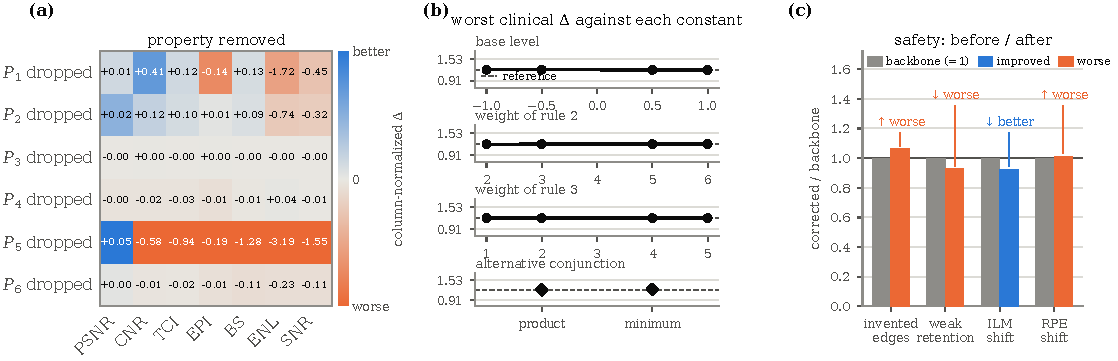
\includegraphics[width=0.86\textwidth]{figures/fig_studies.pdf}
\caption{The three studies of the main paper drawn together. Left, removing one clinical property at
a time, in points of the measure. Only $P_5$, $P_1$ and $P_2$ move any measure by more than a quarter
point, so $P_3$, $P_4$ and $P_6$ are close to inert here. Middle, the fourteen variations of the rule
constants, none of which turns a clinical measure negative, with the base allocation level the only
visible effect. Right, the safety analysis, each of the invented edge rate, weak structure retention
and the two boundary shifts shown as the ratio of corrected to backbone value, one meaning unchanged,
the arrow giving the direction and the word whether it is better or worse for that measure. Three
ratios sit on the worse side, though the retinal pigment epithelium shift moves one percent and is
not significant. All panels are the selected NAFNet checkpoint on the same \NImages{} test images.}
\label{fig:supp_studies}
\end{figure*}

\section{The adapted transfer protocol of the original submission}
\label{sec:supp_adapted}

The cross dataset numbers of the original submission were not produced by the no adaptation
protocol the text described. The script that produced them resumed the corrector trained on PKU37
and trained it further on the target dataset in a leave one subject out design. We rerun that
protocol here with the selected NAFNet checkpoint so that the gap between the two protocols can be
read directly, and we describe it exactly.

\subsection{Protocol}
Each fold holds out one subject, seventeen of Duke2013 or fifteen of Duke17 subjects form the
training set, and the held out subject is evaluated once. Training resumes from the PKU37 checkpoint
of the tissue bounded gate setting at seed 0 and runs for fifteen epochs with batch size two. The
backbone weights and its normalisation statistics are frozen. The wrapper and the cooperation head
that reads the backbone features are trainable. The learning rates are $2{\times}10^{-5}$,
$1{\times}10^{-4}$ and $6{\times}10^{-5}$ for the corrector, potential and negotiator, five to ten
times below the PKU37 schedule of Table~\ref{tab:constants}, the fidelity term enters at epoch five,
and an L2 penalty of weight 0.1 holds every trainable weight near its PKU37 value, which is elastic
weight consolidation without the Fisher weighting. A background correction variance penalty of
weight 10 is also active. The checkpoint kept for each fold is the epoch with the highest validation
score, and the validation image of a fold is its held out subject. The adapted numbers are therefore
selected on the subject they are evaluated on and should be read as an upper bound for this
protocol. The same was true of the original submission.

\subsection{Result}
Table~\ref{tab:supp_adapted} gives both target sets, next to the no adaptation result of the same
checkpoint from the main paper.

\begin{table}[!tb]
\centering
\caption{NAFNet, adapted protocol over one leave one subject out fold per subject, against the no
adaptation protocol of Table 3 of the main paper on the same checkpoint. Clinical rows are percentage
change from backbone output to corrected output. The spread is the standard deviation across
subjects, the count is the number of subjects on which the measure improved, and $p$ is a two sided
Wilcoxon signed rank test on the paired per subject values.}
\label{tab:supp_adapted}
\footnotesize
\begin{tabular}{lrrrr}
\toprule
Measure & No adaptation & Adapted & Improved & $p$ \\
\midrule
\multicolumn{5}{l}{\textit{Duke17, 16 subjects}} \\
$\Delta$PSNR (dB) & $-0.17$ & $-0.23 \pm 0.44$ & 6 of 16 & 0.093 \\
$\Delta$CNR & $+7.51$ & $+10.68 \pm 1.55$ & 16 of 16 & $3.1{\times}10^{-5}$ \\
$\Delta$TCI & $+4.00$ & $+2.69 \pm 4.16$ & 12 of 16 & 0.018 \\
$\Delta$EPI & $+1.37$ & $+1.49 \pm 0.78$ & 15 of 16 & $6.1{\times}10^{-5}$ \\
$\Delta$BS & $+4.15$ & $+4.13 \pm 5.18$ & 13 of 16 & 0.0017 \\
$\Delta$ENL & $+21.35$ & $+24.29 \pm 17.72$ & 15 of 16 & $6.1{\times}10^{-5}$ \\
$\Delta$SNR & $+5.43$ & $+2.95 \pm 8.97$ & 9 of 16 & 0.50 \\
\midrule
\multicolumn{5}{l}{\textit{Duke2013, 18 subjects}} \\
$\Delta$PSNR (dB) & $-0.35$ & $-0.45 \pm 0.47$ & 4 of 18 & 0.0016 \\
$\Delta$CNR & $+7.37$ & $+15.43 \pm 4.09$ & 18 of 18 & $7.6{\times}10^{-6}$ \\
$\Delta$TCI & $+1.41$ & $+5.15 \pm 3.75$ & 17 of 18 & $1.5{\times}10^{-5}$ \\
$\Delta$EPI & $+0.85$ & $+0.90 \pm 0.89$ & 15 of 18 & 0.00084 \\
$\Delta$BS & $+0.51$ & $+2.96 \pm 2.97$ & 14 of 18 & 0.0010 \\
$\Delta$ENL & $+28.80$ & $+9.23 \pm 28.61$ & 8 of 18 & 0.80 \\
$\Delta$SNR & $+9.29$ & $-5.29 \pm 13.97$ & 3 of 18 & 0.010 \\
\bottomrule
\end{tabular}
\end{table}

Two things hold on both scanners. Adaptation raises contrast, by 3.2 points on Duke17 and 8.1 on
Duke2013, and every subject improves. Adaptation also costs fidelity and signal to noise ratio
relative to the frozen model, a further 0.06 and 0.10 dB, with one and two subjects losing more than
1 dB, and a signal to noise ratio 2.5 and 14.6 points lower. The mean absolute correction rises from
0.0104 to 0.0121 on Duke17 and from 0.0118 to 0.0164 on Duke2013. The other measures do not agree
between the two sets. On Duke17 the tissue contrast index falls from $+4.0$ to $+2.7$ percent while
the speckle measure rises, and no measure falls below zero, although the signal to noise ratio is no
longer significant. On Duke2013 the tissue contrast index, edge preservation and boundary sharpness
all rise, the speckle measure changes on eight subjects one way and ten the other and is not
significant, and the signal to noise ratio falls by 5.3 percent, a decrease on fifteen of eighteen
subjects that is significant at the one percent level.

We draw one conclusion. Adaptation on fifteen to seventeen images of the target scanner reliably
improves one measure, contrast, which the frozen model already improves on both sets. It pays for
that in fidelity and signal to noise ratio on both sets, its effect on the remaining measures
changes direction between two scanners, and it does so from a checkpoint selected on the held out
subject. The frozen model gives six positive measures on both sets with no fitting on the target
data, and it is the protocol the main paper reports and the one we recommend.


\end{document}
